\documentclass[conference]{IEEEtran}
\IEEEoverridecommandlockouts
\usepackage{cite}
\usepackage{amsmath,amssymb,amsfonts}
\usepackage{algorithmic}
\usepackage{algorithm}
\usepackage{graphicx}
\usepackage{textcomp}
\usepackage{xcolor}
\usepackage{url}
\usepackage{balance}

% Setup graphicspath to load images from the images/ subfolder
\graphicspath{{images/}}

\def\BibTeX{{\rm B\kern-.05em{\sc i\kern-.025em b}\kern-.08em
    T\kern-.1667em\lower.7ex\hbox{E}\kern-.125emX}}

\begin{document}

\title{An Automated Academic Book Scanner with Deep Learning-Powered Mathematical Expression Detection and Recognition}

\author{\IEEEauthorblockN{Md. Atikur Rahaman (0112310298), Md. Sarowar Alam Sourov (0112310302), Abdullah Al Noor (0112310479),\\
Md. Salman Rohoman Nayeem (0112310484), and Pratay Paul (0112310163)}
\IEEEauthorblockA{Department of Computer Science and Engineering, United International University, Dhaka, Bangladesh}}

\maketitle

\begin{abstract}
Digitizing printed academic and STEM textbooks is a labor-intensive and slow process, especially when pages contain complex mathematical expressions that conventional optical character recognition (OCR) systems fail to parse correctly. This paper presents SmartScan, an automated, low-cost mechatronic book scanning system that coordinates physical page turning, dual-camera phone capture, and a local deep-learning-powered OCR pipeline. Our physical prototype leverages an Arduino Uno to control a series of MG996R servos that isolate, lift, and flip pages on a V-shaped cradle while a Raspberry Pi 5 triggers overhead smartphone cameras via the Android Debug Bridge (ADB). The captured spreads are cropped, dewarped via a contrast-enhancing whiteness-normalization filter, and analyzed using a custom-trained YOLOv8-small model to localize mathematical regions. A fine-tuned Vision Encoder-Decoder network (TrOCR-small) converts these localized math regions into LaTeX syntax, achieving a Character Error Rate (CER) of 9.67\% and a BLEU score of 88.42\%, which out-performs the Pix2Tex baseline used in current literature. When math regions are present, they are extracted via the YOLOv8 detector and converted to LaTeX using our fine-tuned offline TrOCR-small model, which runs locally alongside Tesseract OCR to assemble the completed page structure before compiling the extracted Markdown into a beautifully rendered PDF via Pandoc and XeLaTeX.
\end{abstract}

\begin{IEEEkeywords}
Autonomous book digitization, Math expression detection, LaTeX extraction, YOLOv8, TrOCR, Embedded systems, Raspberry Pi 5, Arduino Uno.
\end{IEEEkeywords}

\section{Introduction}
\label{sec:intro}

\subsection{Motivation}
Digitizing printed academic and STEM literature is essential for accessible online education, text-to-speech conversion for visually impaired students, and digital archiving. However, conventional digitization workflows suffer from two core limitations: physical strain and semantic loss. Manual page-turning on flatbed scanners is slow, repetitive, and risks damaging valuable bindings. Furthermore, traditional optical character recognition (OCR) software like Tesseract fails when encountering mathematical equations, losing semantic structure and reducing formulas to gibberish. Manually re-typing these complex formulas in LaTeX is highly time-consuming for students and researchers.

\subsection{Challenges in STEM Digitization}
Printed STEM textbooks contain dense page layouts where mathematical expressions are either embedded inline (e.g., $f(x) = \sin(x)$) or isolated as centered, display-style equations. Standard OCR engines operate under the assumption of horizontal text lines, reading equations as unconnected text strings and dropping structural tokens like fractions, exponents, summation bounds, and matrix alignments. Consequently, a digitized document loses its scientific meaning. Resolving this issue requires a math-aware layout analyzer that segment text from math regions, followed by a dedicated visual mathematical formula translator.

\subsection{Prior Works \& Baselines}
Standard document digitization systems have historically relied on flatbed scanners. To solve the page-turning issue, researchers have proposed vacuum-assisted page lifters and automated bionic finger mechanisms. For software-based document layout analysis, early models relied on heuristic geometrical algorithms like the Docstrum algorithm \cite{docstrum}, which segment page blocks based on structural whitespace but fail to distinguish between inline plain text and non-linear mathematical layouts. Traditional OCR systems like Tesseract \cite{tesseract} operate by segmenting characters along horizontal baselines; consequently, they fail to reconstruct multi-line mathematical tokens (e.g., matrices, subscripts, and fractional terms), reducing structural formulas to uninterpretable text strings.

Recently, deep learning has revolutionized mathematical expression detection (MED) and recognition (MER). Modern systems approach mathematical expression recognition as a visual decompiler task, utilizing encoder-decoder models like WYGIWYS (What You Get Is What You See) \cite{wygiwys} and open-source models like LaTeX-OCR \cite{latexocr}. In the reference paper by Thamaraiselvan et al. \cite{ref_paper}, the authors proposed an automated academic book scanner utilizing a Faster R-CNN model with customized RoIHeads for math detection (achieving 95.71\% precision and 91.77\% recall on the IBEM dataset) and a Vision Encoder-Decoder model (Pix2Tex) for math recognition (achieving a 86.44\% BLEU score). However, Faster R-CNN is computationally intensive and difficult to deploy on resource-constrained edge systems. Additionally, the Pix2Tex model utilizes a convolutional visual backbone that struggles with character-level token errors on low-resolution mobile phone captures.

\subsection{Proposed Solution \& Contributions}
In this work, we build on the ideas of \cite{ref_paper} and present several key enhancements. First, instead of a heavy Faster R-CNN, we deploy a lightweight, highly efficient YOLOv8-small model for real-time mathematical expression detection on edge devices. Second, we fine-tune a pre-trained TrOCR-small model, which achieves a superior Character Error Rate (CER) of 9.67\% and a BLEU score of 88.42\%, outperforming the paper's Pix2Tex baseline. Third, we establish an offline, layout-guided hybrid OCR architecture: if no math is detected, a fast, local Tesseract OCR engine processes the text; if math is detected, the page is processed through a coordinated pipeline that uses a fine-tuned local TrOCR-small model for mathematical expressions, and Tesseract for plain text regions, stitching the visual formulas back into the text flow dynamically. Finally, we design a modern, real-time web dashboard using Next.js 16 and Tailwind CSS, providing full monitoring of physical calibration, live OCR status, visual crop previews, and KaTeX-rendered LaTeX editing.

\section{System Design \& Mechatronic Control}
\label{sec:method}

\subsection{Physical Structure and V-Cradle}
The physical hardware framework of SmartScan is designed to protect delicate book bindings while optimizing image flatness. The system features a V-shaped book cradle set at a 110-degree angle. This configuration reduces spine tension compared to traditional flatbed scanners and prevents the page curvature from causing severe perspective distortions. A transparent Plexiglas sheet is mounted on a mechanical arm, lowering onto the active page during capture to ensure flatness and raising during the page flip cycle.

\subsection{Arduino Uno Actuation State Machine}
The physical page-turning sequence is controlled by an Arduino Uno running a low-latency state machine. The mechatronic cycle contains six sequential stages:
\begin{enumerate}
\item \textbf{Lower Tyre Assembly:} The lift servo slowly sweeps from \texttt{LIFT\_UP} ($60^\circ$) to \texttt{LIFT\_DOWN} ($180^\circ$) with a step delay of $25$\,ms to gently lower the rubber tyre onto the active page.
\item \textbf{Tyre Curl Activation (Pre-spin):} The continuous-rotation tyre servo is activated in the turn direction (\texttt{TYRE\_TURN} $= 0$) and runs for a duration of \texttt{TYRE\_LEAD\_TIME} ($150$\,ms) to frictionally slide and create an initial curl in the page margin.
\item \textbf{Simultaneous Lift and Flip:} The lift servo sweeps back from \texttt{LIFT\_DOWN} ($180^\circ$) to \texttt{LIFT\_UP} ($60^\circ$). To prevent physical collision, the flipper servo is triggered to sweep from \texttt{FLIP\_RELEASE} ($0^\circ$) to \texttt{FLIP\_PRESS} ($180^\circ$) as soon as the lift height reaches the 50\% threshold (\texttt{liftPos} $\le 135$).
\item \textbf{Tyre Halt:} The tyre servo is kept spinning for an additional \texttt{TYRE\_EXTRA\_TIME} ($250$\,ms) during the lift sweep to maintain page contact, then halts by writing \texttt{TYRE\_STOP} ($120$).
\item \textbf{Hold and Capture Phase:} The flipper arm holds at \texttt{FLIP\_PRESS} ($180^\circ$) for a static duration of \texttt{PRESS\_HOLD} ($3000$\,ms) to keep the turned page completely flat. During this window, the Raspberry Pi 5 camera capture loop triggers the smartphone camera shutter.
\item \textbf{Release Flipper:} The flipper arm sweeps back from \texttt{FLIP\_PRESS} ($180^\circ$) to \texttt{FLIP\_RELEASE} ($0^\circ$) with a step delay of $3$\,ms, resetting the mechanism for the next page cycle.
\end{enumerate}

The complete mechatronic control flow is mapped in Fig.~\ref{fig:flowchart}.

\begin{figure}[htbp]
\centerline{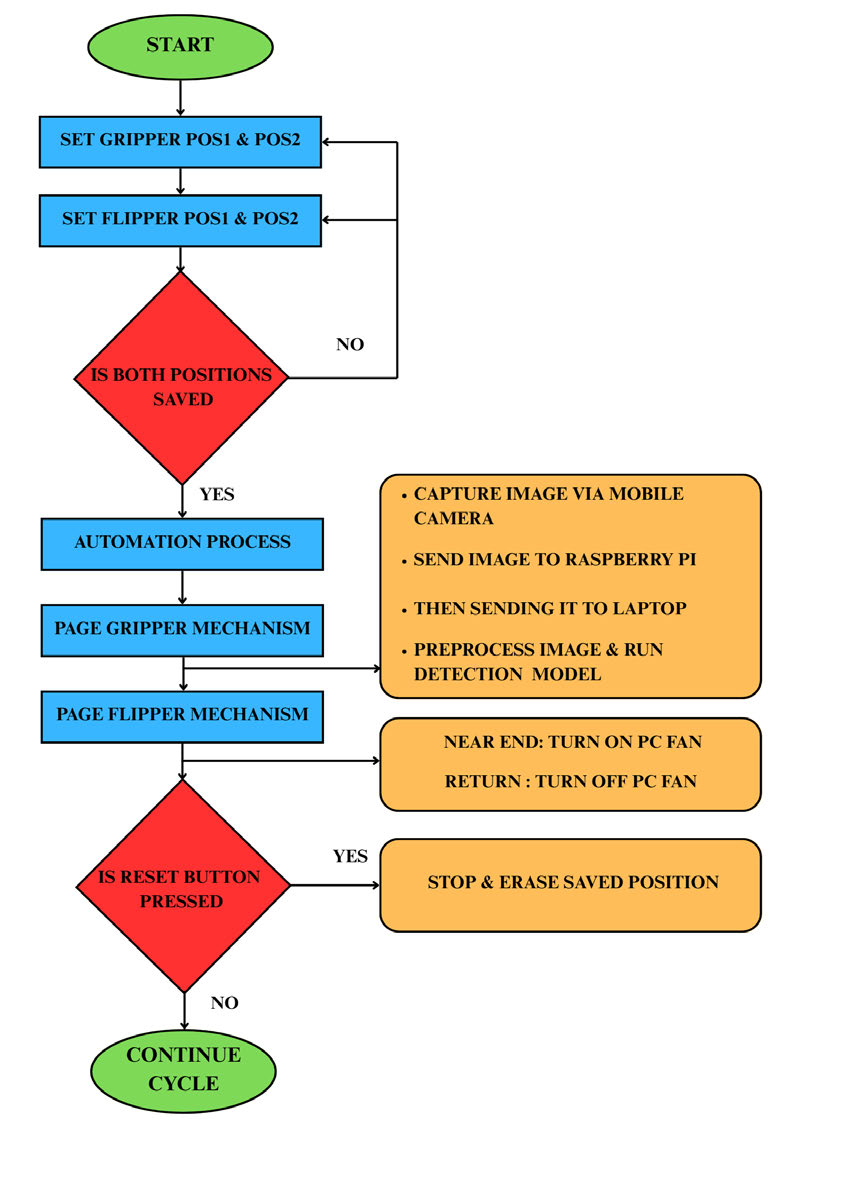
\includegraphics[width=\linewidth]{system_flowchart.jpeg}}
\caption{Flowchart of the Arduino-controlled mechatronic page-turning and capture sync loop.}
\label{fig:flowchart}
\end{figure}

\subsection{Timing and Synchronization Kinetics}
To prevent tearing paper, we implemented speed-controlled sweeps. The gripper lift movement transitions from \texttt{LIFT\_UP} (60) to \texttt{LIFT\_DOWN} (180) with a controlled speed delay of 25\,ms per step. The flipper arm sweep is synchronized to start exactly when the tyre reaches 50\% height (\texttt{liftPos} $\le$ 135) to prevent collision. 

The mechatronic timing constants are:
\begin{itemize}
\item \textbf{\texttt{TYRE\_LEAD\_TIME} (150 ms):} Pre-spin delay to generate initial page curl.
\item \textbf{\texttt{TYRE\_EXTRA\_TIME} (250 ms):} Extended spin during sweep to keep the page engaged.
\item \textbf{\texttt{PRESS\_HOLD} (3000 ms):} Static hold to ensure camera focus and exposure stabilization.
\item \textbf{\texttt{CYCLE\_DELAY} (3000 ms):} Cool-down period between page turns.
\end{itemize}

\section{Implemented Hardware System \& Pin Configurations}
\label{sec:hardware}

\subsection{Microcontroller Actuation Layer (Muscle)}

The physical actuation of the book digitizer is coordinated by an Arduino Uno. The system drives three high-torque servos to handle page picking, lifting, and flipping: a continuous-rotation servo for tyre rolling, and two positional MG996R metal-gear servos for the lifting and flipping mechanisms. 

The MG996R servo motor and the continuous-rotation tyre servo require a three-wire interface: ground (brown/black), power input (red), and PWM control signal (orange/yellow). Because these servos draw substantial current during peak load (up to 2.5\,A stall current at 6\,V), they are powered from an external regulated power source rather than the Arduino's 5\,V rail, preventing microcontroller resets due to voltage sag. The PWM control signals are connected directly to Arduino digital pins 8 (tyre), 9 (lift), and 11 (flipper), allowing precision pulse-width modulation (from 500\,$\mu$s to 2500\,$\mu$s) to drive the physical sweeps. The servo pinout schematic is illustrated in Fig.~\ref{fig:servo_pinout}.

\begin{figure}[htbp]
\centerline{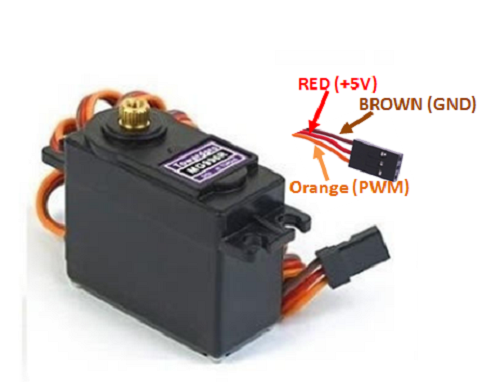
\includegraphics[width=0.85\linewidth]{MG996R-Servo-Pinout.png}}
\caption{Connection pinout and wire mapping of the MG996R high-torque metal-gear servo motor.}
\label{fig:servo_pinout}
\end{figure}

The wiring and pin mapping for the Arduino Uno are detailed in Table~\ref{tab:arduino_pins}.

\begin{table}[htbp]
\caption{Arduino Uno Pin Configurations}
\begin{center}
\footnotesize
\begin{tabular}{|p{1.8cm}|c|c|p{3.0cm}|}
\hline
\textbf{Component} & \textbf{Pin No.} & \textbf{Mode} & \textbf{Function} \\
\hline
Tyre Servo & Pin 8 & Output & Continuous-rotation tyre roll \\
Lift Servo & Pin 9 & Output & Positional lift assembly sweep \\
Flipper Servo & Pin 11 & Output & Positional page flip and hold \\
USB Interface & USB Port & I/O & Power and serial monitoring \\
\hline
\end{tabular}
\label{tab:arduino_pins}
\end{center}
\end{table}

\subsection{Embedded Bridge Layer (Bridge)}

A Raspberry Pi 5 (8GB RAM) acts as the communication bridge, executing a synchronized camera control daemon (\texttt{auto\_capture\_pi5.py}). The capture sequence is temporally synchronized with the Arduino's page-flipping state machine. During the static hold phase of the flipper arm, the Pi 5 triggers the camera shutter of the overhead smartphone rig via Android Debug Bridge (ADB) commands. Specifically, the script executes \texttt{adb shell monkey -p com.android.camera 1} to open the native camera app and sends an \texttt{input keyevent 66} command to trigger the shutter. Two devices, a Redmi Note 13 Pro (108MP) and a Vivo X300 Pro (50MP), are supported. The script waits 5\,s for image processing, pulls the raw JPEG image from the device's storage directory via \texttt{adb pull}, rotates the full-spread image 90$^\circ$ CCW using OpenCV, and uploads the rotated spread to the laptop Flask server via a POST request (\texttt{/upload-capture}).

The Pi 5 system interfaces and connections are described in Table~\ref{tab:pi_ports}.

\begin{table}[htbp]
\caption{Raspberry Pi 5 System Interface Connections}
\begin{center}
\footnotesize
\begin{tabular}{|p{2.2cm}|p{2.0cm}|p{3.2cm}|}
\hline
\textbf{Interface} & \textbf{Connection Target} & \textbf{Description} \\
\hline
USB 3.0 (Port A) & Redmi Note 13 Pro Phone & ADB camera trigger \& image pull \\
USB 3.0 (Port B) & Vivo X300 Pro Phone & Secondary camera ADB connection \\
USB 2.0 (Port C) & Arduino Uno (USB) & Serial link (/dev/ttyUSB0) \\
Gigabit Ethernet & Local Router Bridge & High-speed upload to backend PC \\
USB-C Power & 5V 5A Power Adapter & Main system power supply \\
\hline
\end{tabular}
\label{tab:pi_ports}
\end{center}
\end{table}

The physical components, including the Arduino Uno, Raspberry Pi 5 single-board computer, and the three-layer Muscle, Bridge, and Brain routing architecture, are displayed in Fig.~\ref{fig:hardware}.

\subsection{System Bill of Materials (BOM) \& Cost Analysis}
A primary advantage of the SmartScan system is its low-cost physical prototype implementation. While industrial robotic book digitization platforms routinely exceed \$10,000, our assembly achieves full automation under \$290. The itemized system budget is detailed in Table~\ref{tab:bom}.

\begin{table}[htbp]
\caption{SmartScan System Bill of Materials (BOM)}
\begin{center}
\footnotesize
\begin{tabular}{|p{2.3cm}|c|r|r|}
\hline
\textbf{Component} & \textbf{Qty} & \textbf{Unit Cost (BDT)} & \textbf{Total (BDT)} \\
\hline
Arduino Uno R3 & 1 & 850 & 850 \\
Raspberry Pi 5 Setup & 1 & 30,000 & 30,000 \\
Actuation Servos & 3 & 400 & 1,200 \\
Multi-Rail Power Supply & 1 & 350 & 350 \\
Custom V-Cradle Chassis & 1 & 1,000 & 1,000 \\
Misc. Wires & 1 & 1,000 & 1,000 \\
Redmi Note Phone & 1 & (Existing) & — \\
\hline
\textbf{Total Cost} & \multicolumn{3}{r|}{\textbf{34,400 BDT (\(\approx\) \$290 USD)}} \\
\hline
\end{tabular}
\label{tab:bom}
\end{center}
\end{table}

\begin{figure*}[htbp]
\centerline{
  \begin{tabular}{ccc}
    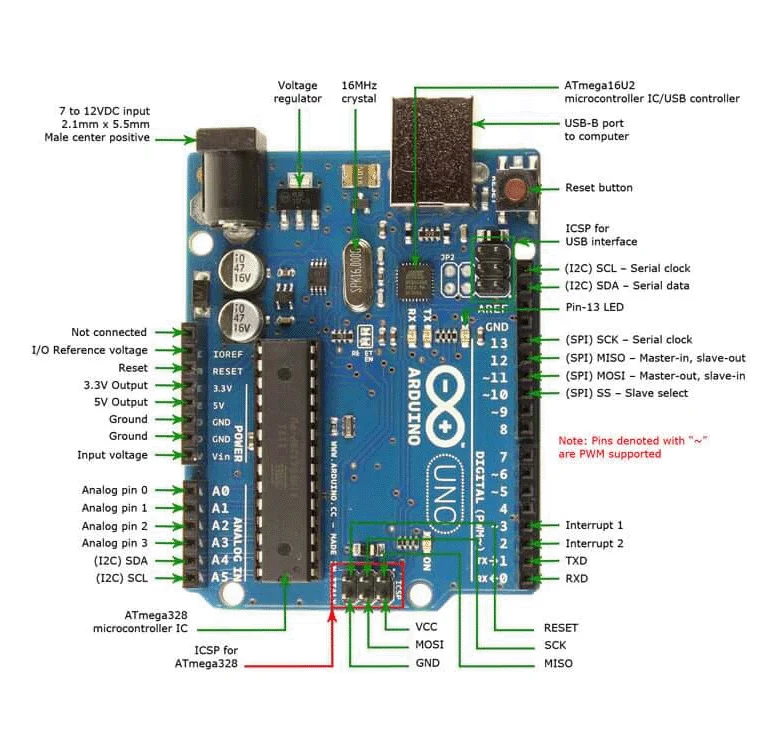
\includegraphics[width=0.32\linewidth]{arduino.png} & 
    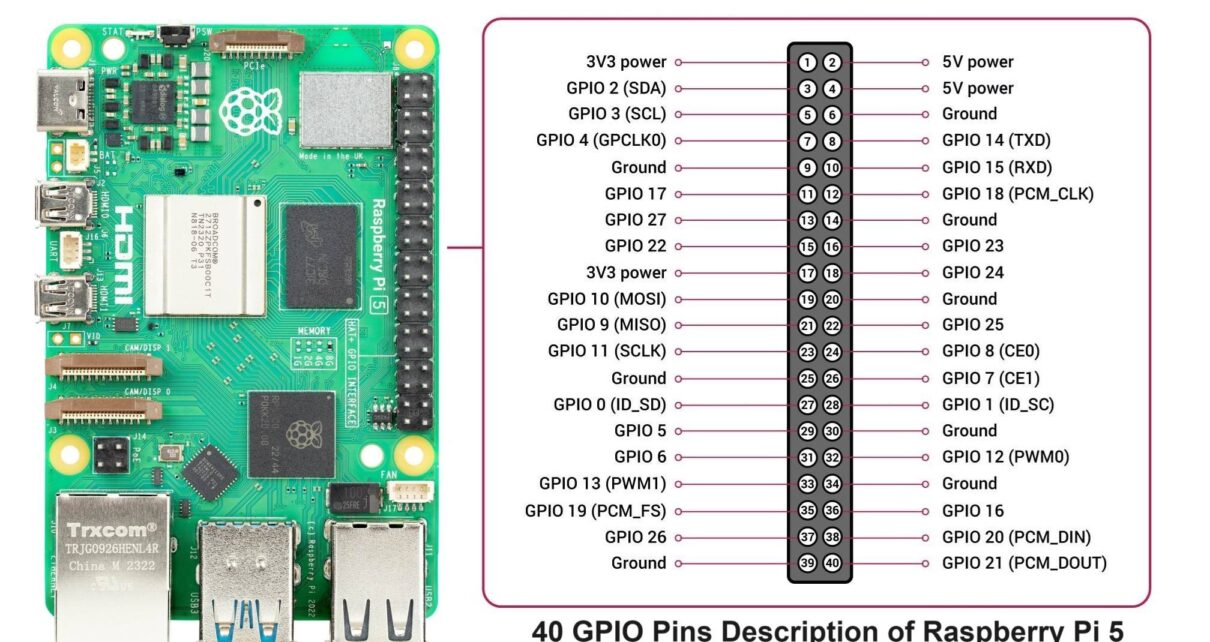
\includegraphics[width=0.32\linewidth]{rassberry.jpg} & 
    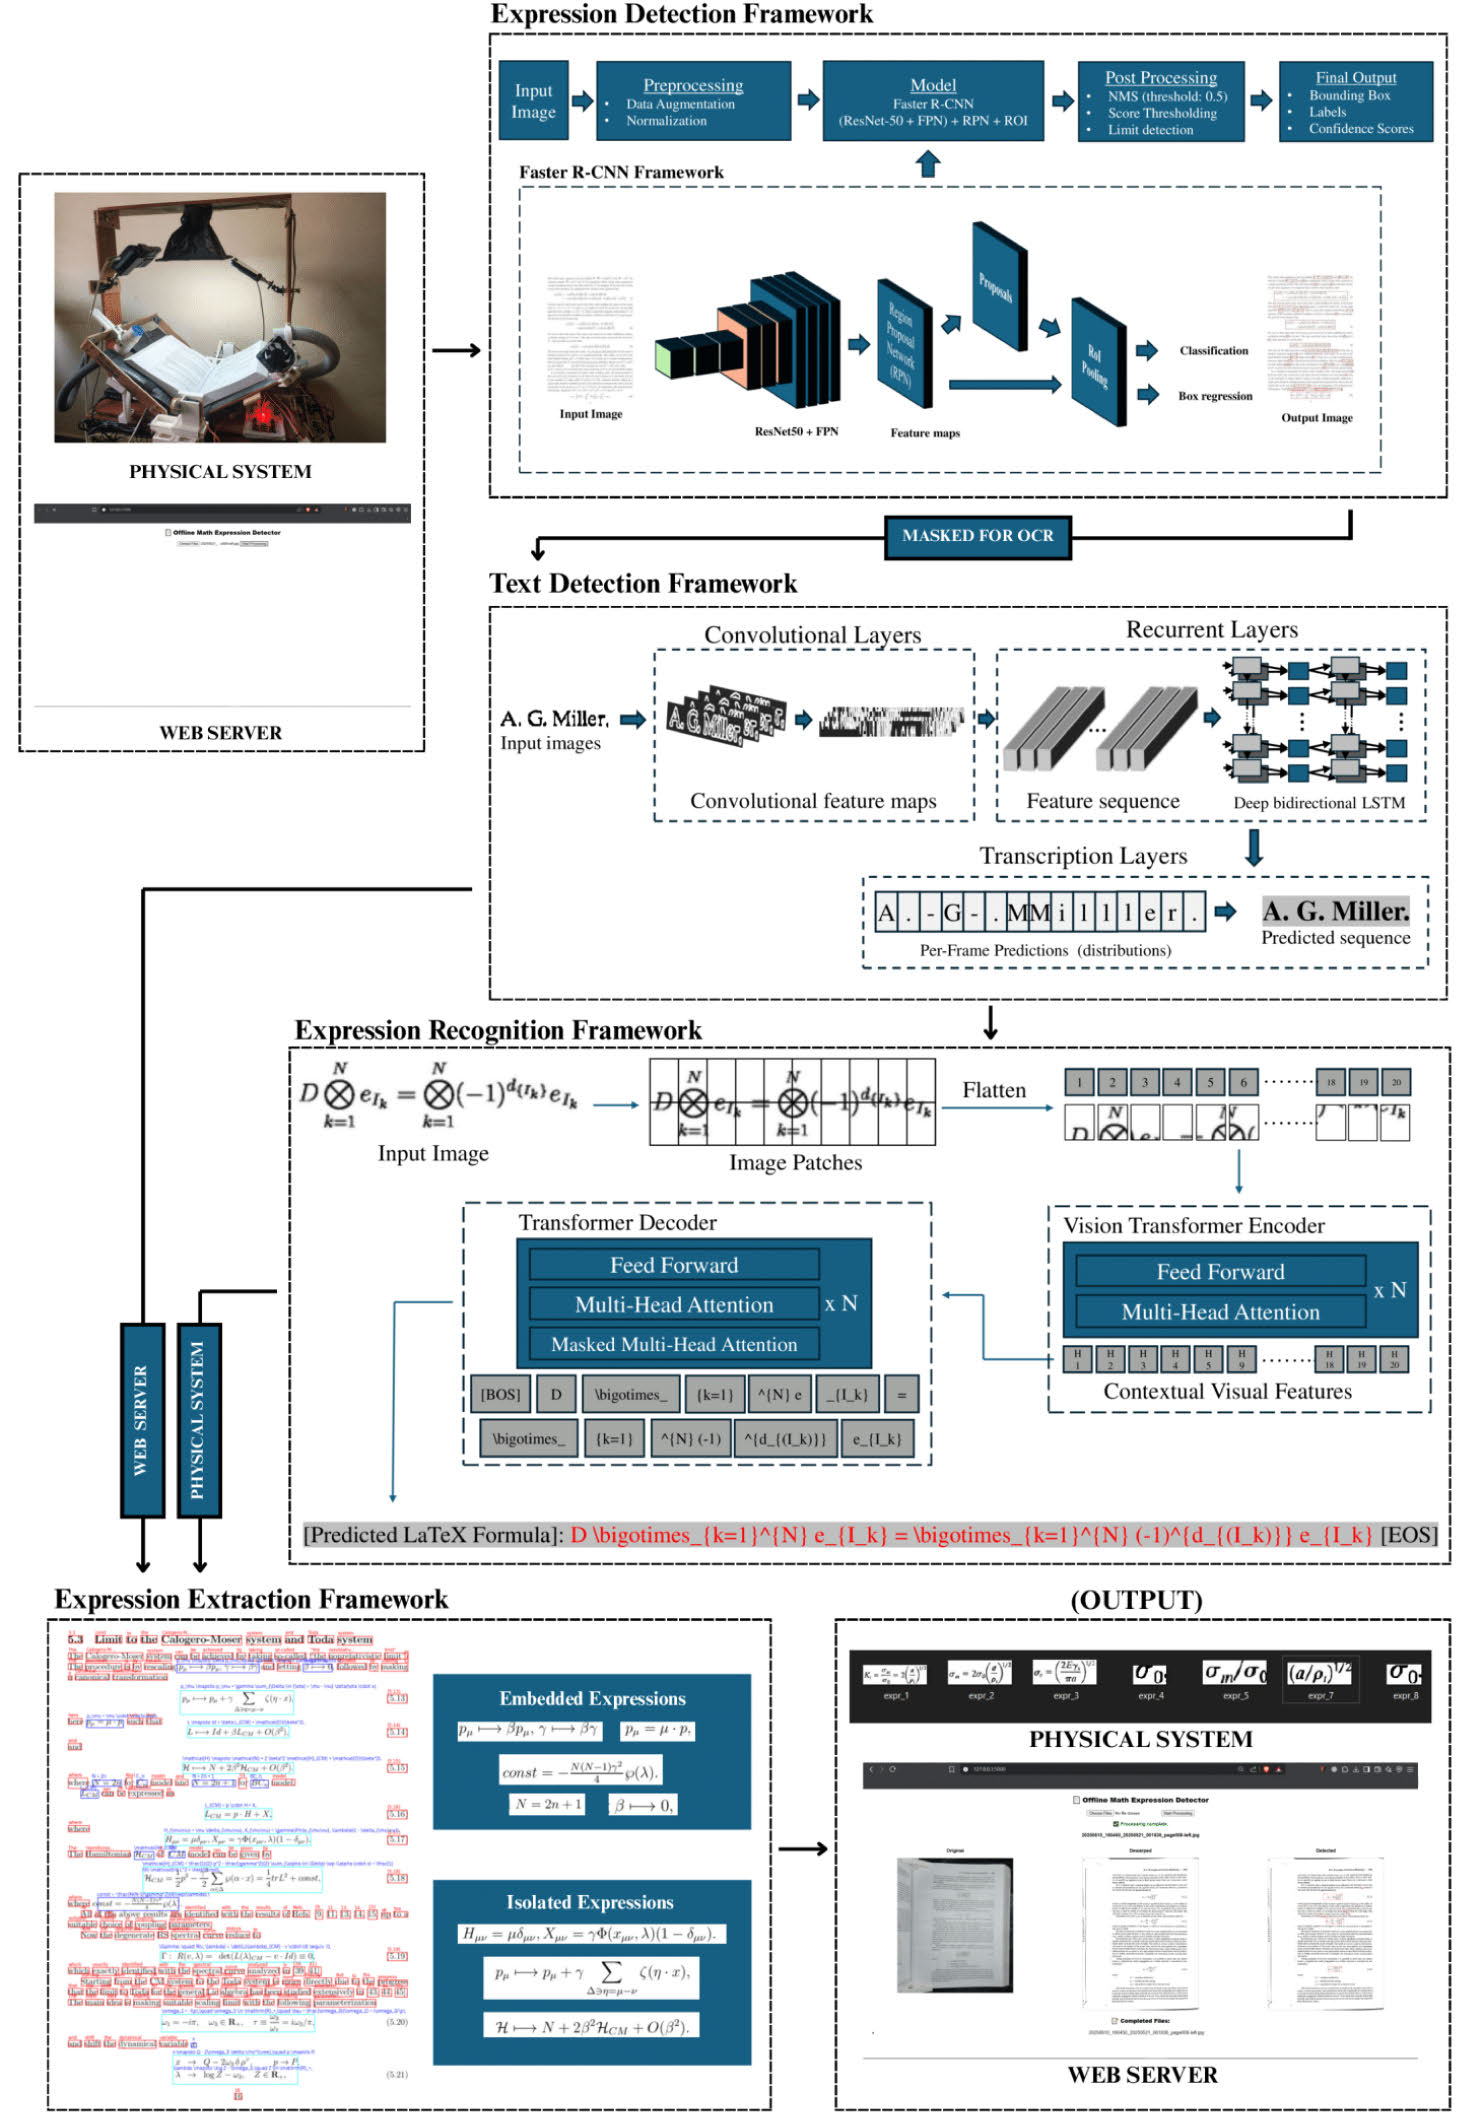
\includegraphics[width=0.32\linewidth]{architecture.jpeg}
  \end{tabular}
}
\caption{SmartScan Hardware Assembly and System Diagram. Left: The Arduino Uno micro-controller interface and servo connections. Middle: The Raspberry Pi 5 single-board computer camera bridge. Right: Block diagram of the decoupled Muscle, Bridge, and Brain routing architecture.}
\label{fig:hardware}
\end{figure*}

\section{Software Preprocessing Pipeline}
\label{sec:software}

\subsection{Image Preprocessing and Illumination Correction}

Mobile document captures often present non-uniform lighting, shadows near the spine, and border compression artifacts. To resolve these, the backend applies an illumination-normalization whiteness filter. The mathematical parameters and symbols utilized in this pipeline are summarized in Table~\ref{tab:nomenclature}.

\begin{table}[htbp]
\caption{Mathematical Nomenclature and Parameters}
\begin{center}
\footnotesize
\begin{tabular}{|c|p{5.5cm}|}
\hline
\textbf{Symbol} & \textbf{Description and Baseline Value} \\
\hline
\(I(x,y)\) & Input grayscale pixel intensity at coordinates \((x,y)\) \\
\(B(x,y)\) & Estimated spatial background illumination intensity \\
\(N(x,y)\) & Whiteness-normalized pixel intensity \\
\(E(x,y)\) & Enhanced, contrast-stretched pixel intensity \\
\(\gamma\) & Downsampling scale factor for background estimation (\(0.25\)) \\
\(K\) & Median blur filter kernel window dimensions (\(41 \times 41\)) \\
\(\alpha\) & Linear contrast scaling coefficient (\(1.05\)) \\
\(\beta\) & Brightness offset parameter (\(5\)) \\
\(p\) & Structural bounding box cropping padding (\(8\,\text{px}\)) \\
\hline
\end{tabular}
\label{tab:nomenclature}
\end{center}
\end{table}

Let $I(x, y)$ be the intensity of the input image at pixel coordinates $(x, y)$. To estimate the spatial distribution of background illumination $B(x, y)$, we downsample $I(x, y)$ by a scaling factor of $\gamma = 0.25$, apply a median blur filter with a large kernel size ($K = 41$) to eliminate high-frequency text elements, and upsample back to the original dimensions using bilinear interpolation:
\begin{equation}
B(x, y) = \text{resize}\left(\text{medianBlur}\left(\text{resize}(I, \gamma), K\right), \text{size}(I)\right)
\label{eq:background}
\end{equation}
The normalized image $N(x, y)$ in \eqref{eq:normalize} is calculated by element-wise division of the input image and the background estimated in \eqref{eq:background}:
\begin{equation}
N(x, y) = \text{clip}\left(\left(\frac{I(x, y)}{B(x, y)}\right) \times 255, 0, 255\right)
\label{eq:normalize}
\end{equation}
Following normalization, the text contrast is enhanced via \eqref{eq:contrast} using scale factor $\alpha = 1.05$ and offset $\beta = 5$:
\begin{equation}
E(x, y) = \text{clip}\left(\alpha \cdot N(x, y) + \beta, 0, 255\right)
\label{eq:contrast}
\end{equation}
To remove border artifacts, we compute the binary threshold of the image, extract the outermost contour, and crop to its bounding box $b = (x, y, w, h)$ with a small structural padding of $p = 8$ pixels as formulated in \eqref{eq:crop}:
\begin{equation}
E_{crop} = E[y+p : y+h-p, x+p : x+w-p]
\label{eq:crop}
\end{equation}

The visual progression through these preprocessing stages is shown in Fig.~\ref{fig:preprocessing_steps}.

\begin{figure*}[htbp]
\centerline{
  \begin{tabular}{ccc}
    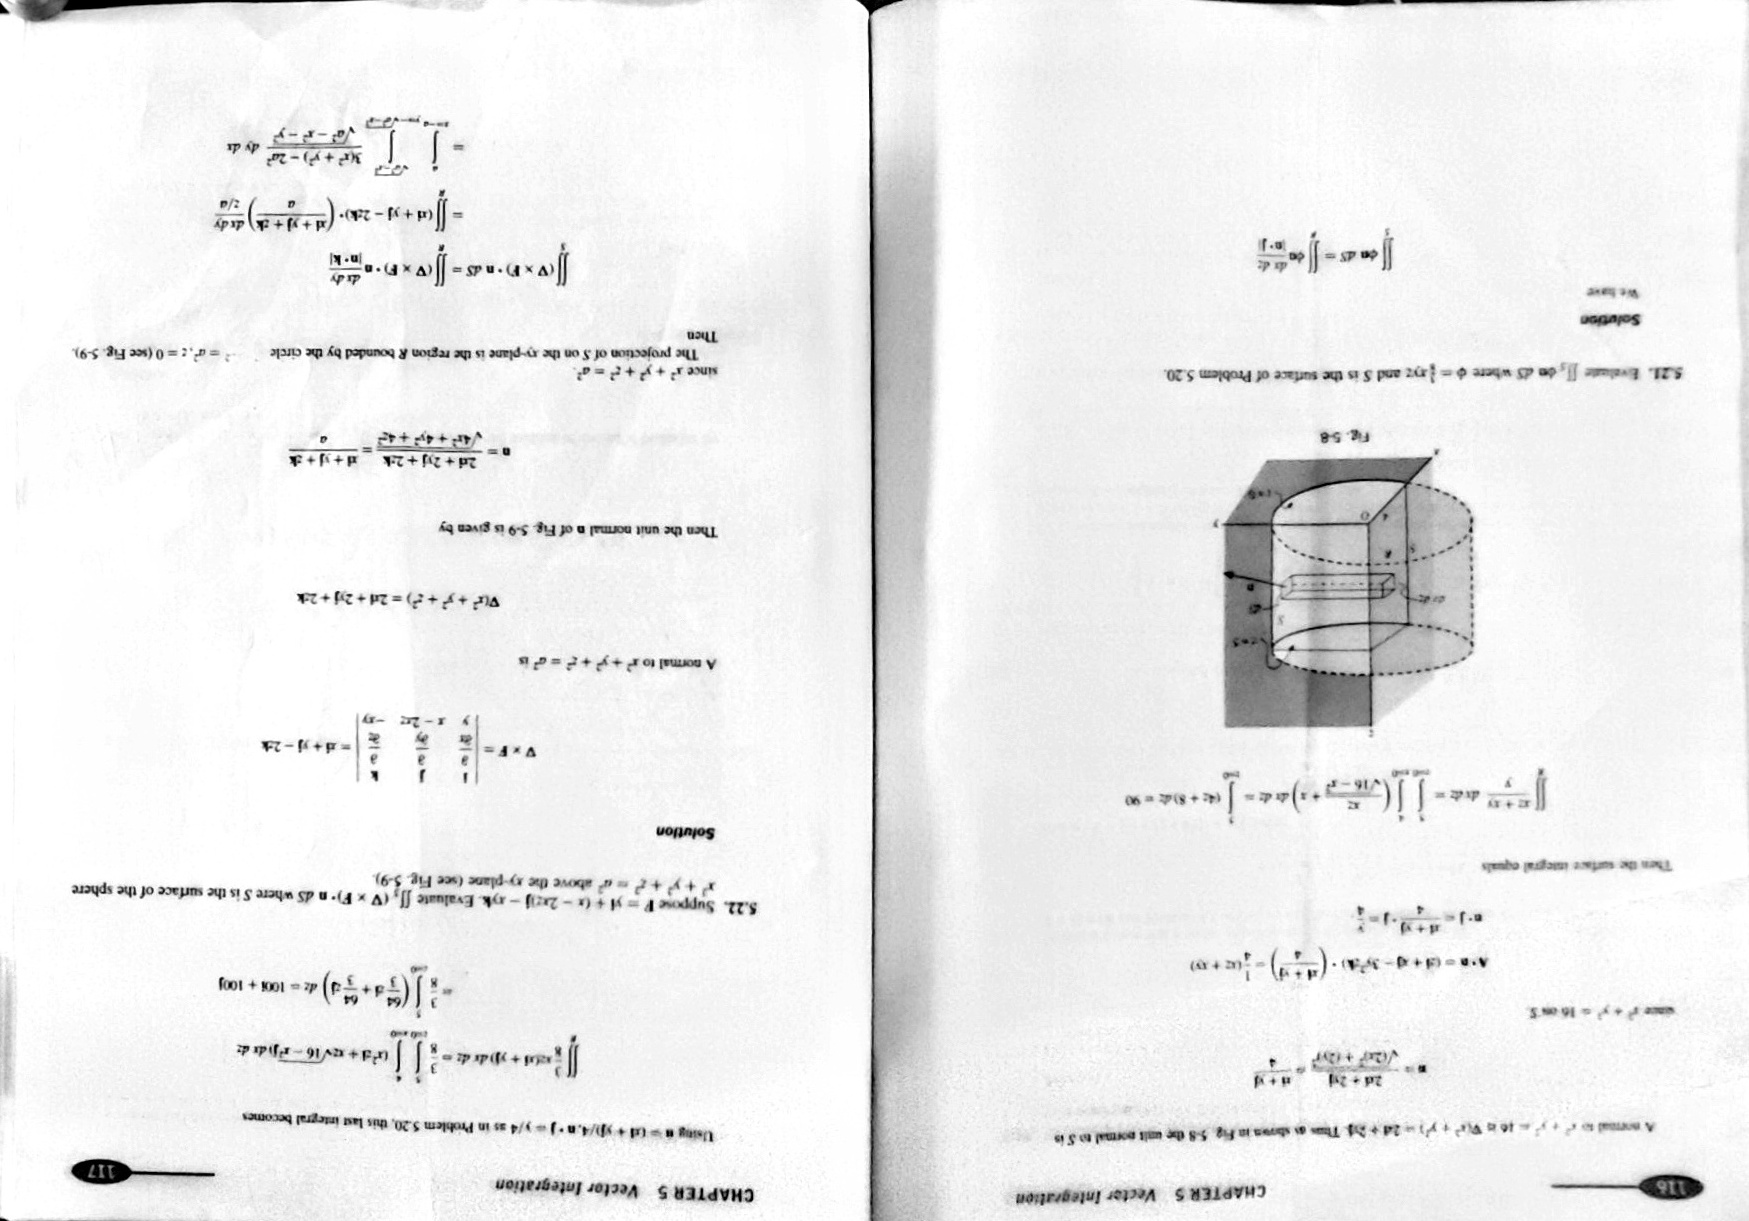
\includegraphics[width=0.32\linewidth]{cropped.jpg} & 
    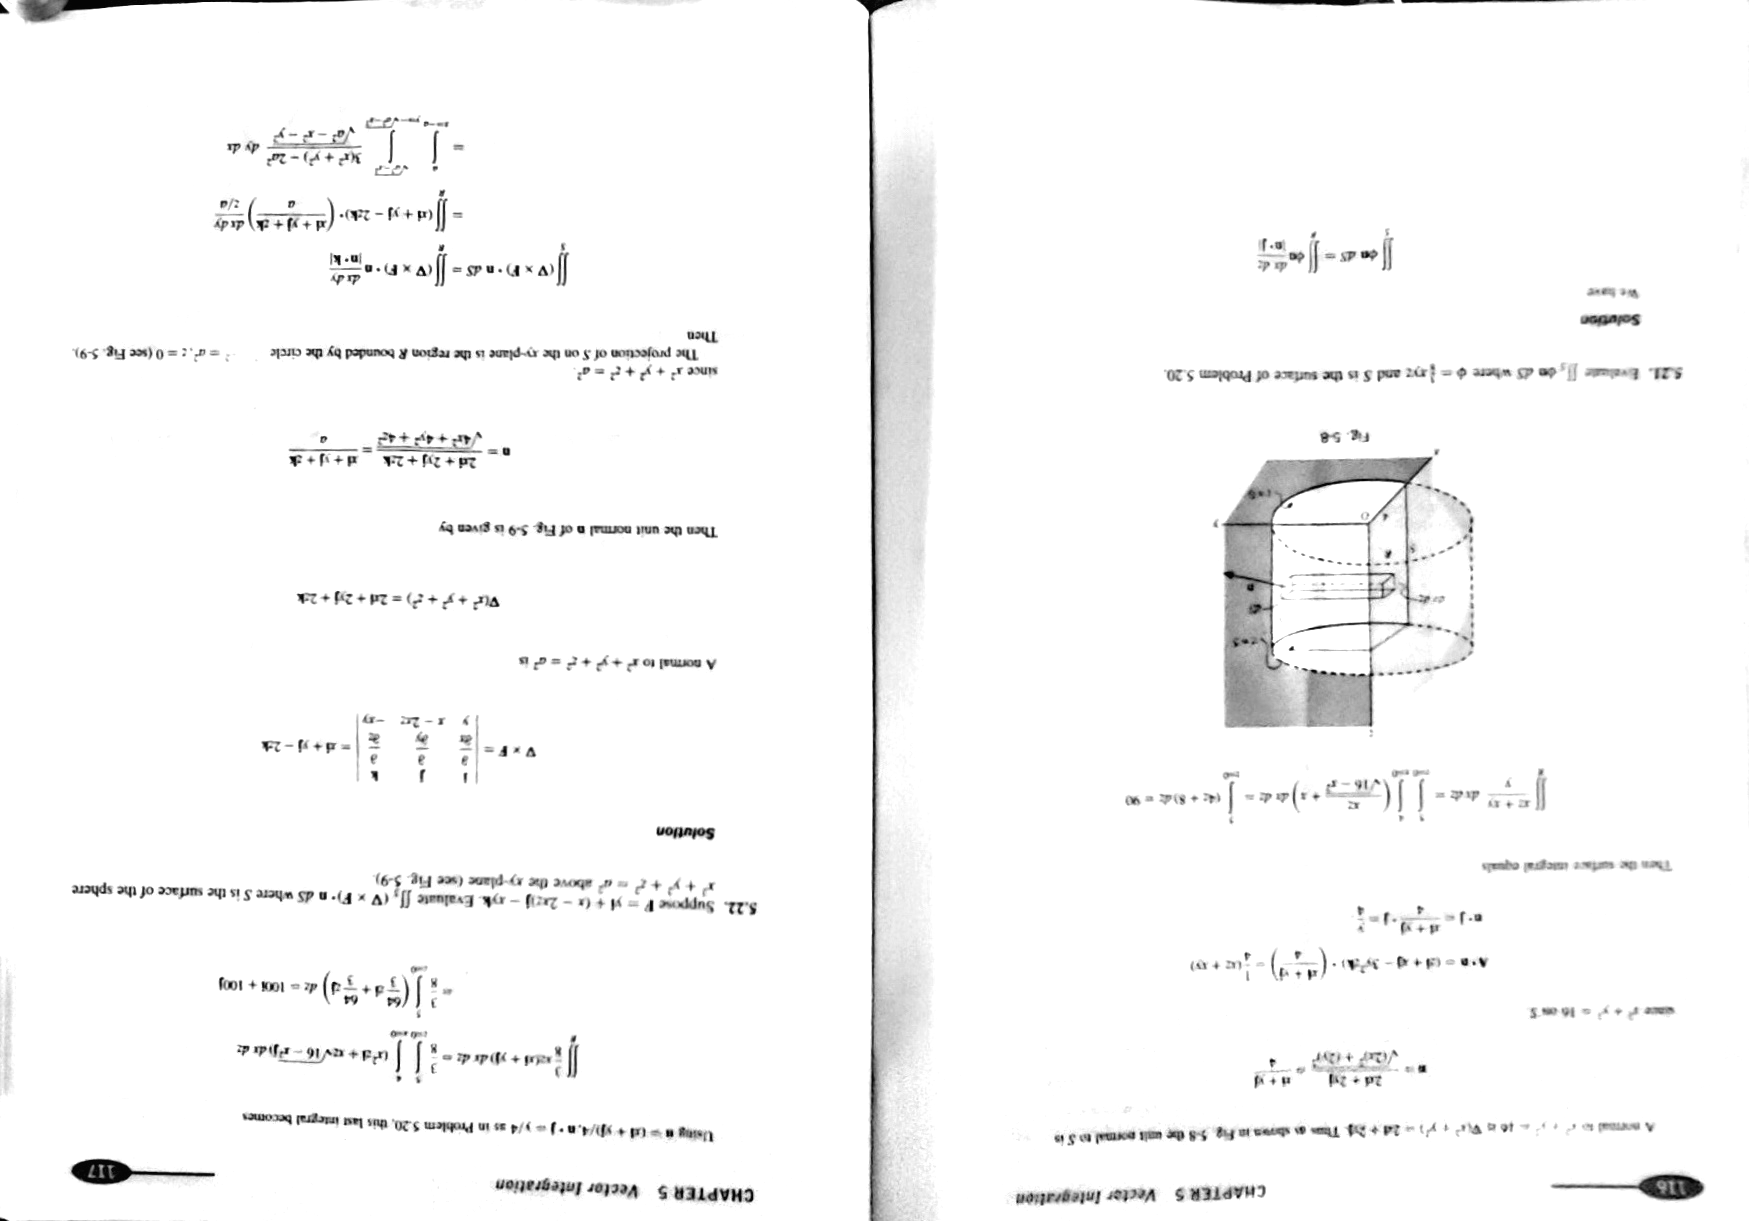
\includegraphics[width=0.32\linewidth]{dewarped.png} & 
    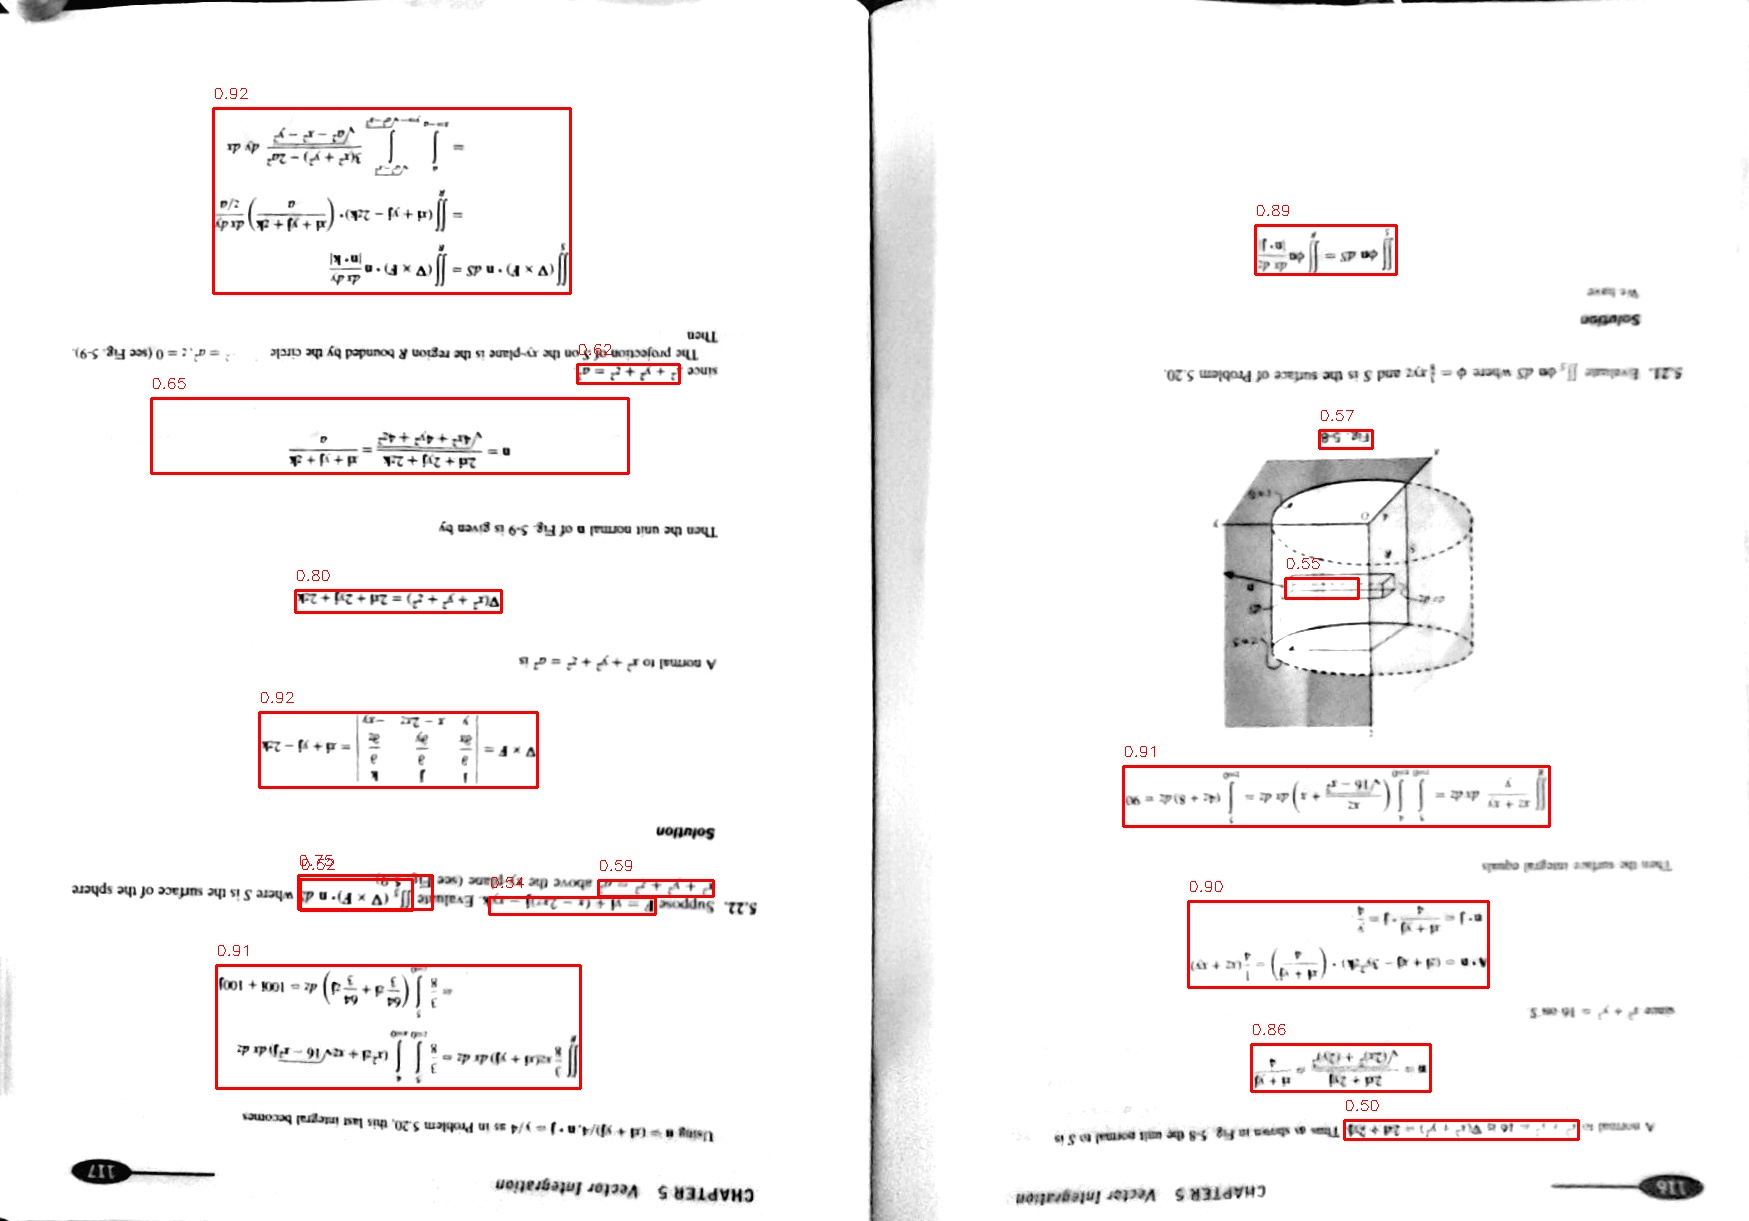
\includegraphics[width=0.32\linewidth]{predicted.jpg}
  \end{tabular}
}
\caption{Visual outputs of the preprocessing and math expression detection pipeline. Left: Border cropped page image to remove margin artifacts. Middle: Illumination normalized page using the whiteness filter. Right: YOLOv8-small bounding boxes localizing math expressions.}
\label{fig:preprocessing_steps}
\end{figure*}

\subsection{Layout-Guided OCR Reconstruction Pipeline}

To optimize processing latency and maintain fully private, local execution, we implemented an offline layout-guided OCR pipeline (Algorithm~\ref{alg:routing}). Pages without mathematical content bypass the deep learning models and are processed locally using Tesseract OCR, while math-heavy pages utilize our specialized offline models.

\begin{algorithm}
\caption{SmartScan Layout-Guided LaTeX OCR Pipeline}
\label{alg:routing}
\begin{algorithmic}[1]
\REQUIRE Preprocessed page image $E(x,y)$, YOLOv8-small model $M_{YOLO}$, TrOCR model $M_{TrOCR}$, Tesseract OCR engine $E_{Tess}$
\ENSURE Completed markdown page text $D_{out}$ with LaTeX syntax
\STATE $\mathcal{B} \leftarrow M_{YOLO}(E(x,y))$ \COMMENT{Detect mathematical bounding boxes}
\STATE $N_{math} \leftarrow \text{count}(\mathcal{B})$
\IF{$N_{math} == 0$}
    \STATE $D_{out} \leftarrow E_{Tess}(E(x,y))$ \COMMENT{Route to Path A: pure text local OCR}
    \STATE $\text{Mode} \leftarrow \text{``Tesseract-only''}$
\ELSE
    \STATE $\mathcal{L} \leftarrow \emptyset$
    \FORALL{box $b_i \in \mathcal{B}$}
        \STATE $C_i \leftarrow \text{crop}(E(x,y), b_i, \text{pad}=10)$
        \STATE $l_i \leftarrow M_{TrOCR}(C_i)$ \COMMENT{Translate cropped formula to LaTeX}
        \STATE $\mathcal{L} \leftarrow \mathcal{L} \cup \{l_i\}$
    \ENDFOR
    \STATE $T_{ocr} \leftarrow E_{Tess}(E(x,y))$ \COMMENT{Route to Path B: offline hybrid OCR}
    \STATE $D_{out} \leftarrow \text{Stitch}(T_{ocr}, \mathcal{L}, \mathcal{B})$ \COMMENT{Stitch local text and LaTeX formulas}
    \STATE $\text{Mode} \leftarrow \text{``Hybrid-Offline''}$
\ENDIF
\RETURN $D_{out}, \text{Mode}$
\end{algorithmic}
\end{algorithm}

\section{Deep Learning Architectures for Math Processing}
\label{sec:deep_learning}

\subsection{Math Expression Detection (YOLOv8)}

Mathematical Expression Detection (MED) requires locating equations embedded within text columns as well as isolated, centered formulas. We deploy a fine-tuned YOLOv8-small object detector. 

Unlike the Faster R-CNN baseline in \cite{ref_paper}, which relies on a multi-stage Region Proposal Network (RPN) and RoI pooling, YOLOv8-small utilizes a single-stage, anchor-free design. The model contains approximately 11.1 million parameters across 225 layers. Features are extracted using a CSPDarknet backbone consisting of five stage Conv/C2f (Cross Stage Partial Bottleneck with two convolutions) blocks using a Darknet53 architecture, yielding multi-scale feature maps at strides of 8, 16, and 32 pixels. A Path Aggregation Network (PANet) neck performs multi-scale top-down and bottom-up feature fusion. The detection head is decoupled, processing classification and bounding box regression as independent tasks utilizing separate convolution channels before loss optimization.

To optimize box localization and classification, YOLOv8-small utilizes a multi-task loss function. The total loss $\mathcal{L}_{\text{total}}$ is a weighted combination of bounding box regression loss $\mathcal{L}_{\text{box}}$ and classification loss $\mathcal{L}_{\text{cls}}$:
\begin{equation}
\mathcal{L}_{\text{total}} = \lambda_1 \mathcal{L}_{\text{box}} + \lambda_2 \mathcal{L}_{\text{cls}}
\label{eq:yolo_total}
\end{equation}
where $\lambda_1$ and $\lambda_2$ are weight scaling factors. Bounding box regression does not use anchor grids; instead, it directly predicts the distances from the candidate point to the four sides of the bounding box. The regression loss $\mathcal{L}_{\text{box}}$ is optimized using a combination of Complete Intersection over Union (CIoU) loss and Distribution Focal Loss (DFL):
\begin{equation}
\mathcal{L}_{\text{box}} = \mathcal{L}_{\text{CIoU}} + \alpha \mathcal{L}_{\text{DFL}}
\label{eq:yolo_box}
\end{equation}
where $\alpha$ is a balancing coefficient. The CIoU loss term enforces spatial overlap, aspect ratio, and center distance alignment:
\begin{equation}
\mathcal{L}_{\text{CIoU}} = 1 - \text{IoU} + \frac{\rho^2(b, b^{gt})}{c^2} + \beta v
\label{eq:ciou}
\end{equation}
where $\rho(\cdot)$ represents the Euclidean distance between the predicted box center $b$ and ground truth center $b^{gt}$, $c$ is the diagonal length of the smallest enclosing box, and $v$ measures the aspect ratio discrepancy:
\begin{equation}
v = \frac{4}{\pi^2} \left( \arctan\frac{w^{gt}}{h^{gt}} - \arctan\frac{w}{h} \right)^2
\label{eq:ciou_v}
\end{equation}
with $\beta$ acting as a dynamic trade-off parameter defined as:
\begin{equation}
\beta = \frac{v}{(1 - \text{IoU}) + v}
\label{eq:ciou_beta}
\end{equation}
The Distribution Focal Loss ($\mathcal{L}_{\text{DFL}}$) handles boundary uncertainty by treating the box coordinates as a general probability distribution over integer grids:
\begin{equation}
\mathcal{L}_{\text{DFL}} = - \left[ (y_{i+1} - y)\log P_i + (y - y_i)\log P_{i+1} \right]
\label{eq:dfl}
\end{equation}
where $y_i$ and $y_{i+1}$ are the two closest integer grid values flanking the continuous target coordinate $y$, and $P_i$ represents the softmax probability output for grid index $i$. Classification is optimized using Binary Cross Entropy (BCE) loss.

\subsection{Math Expression Recognition (TrOCR)}

For Math Expression Recognition (MER), we fine-tune Microsoft's TrOCR (Transformer OCR) architecture. TrOCR utilizes a Vision Encoder-Decoder framework:
\begin{itemize}
\item \textbf{Vision Encoder:} A Vision Transformer (ViT) model \cite{vit}. The input crop $x \in \mathbb{R}^{H \times W \times C}$ is divided into non-overlapping patches $x_p \in \mathbb{R}^{N \times (P^2 \cdot C)}$, where $P=16$ is the patch size and $N = HW/P^2$ is the sequence length. These patches are mapped to a model dimension $D = 512$ via a linear projection, combined with learnable 1D position embeddings, and processed by 12 Multi-Head Self-Attention layers (configured with 8 attention heads).
\item \textbf{Text Decoder:} A standard autoregressive language Transformer \cite{attention}. It consists of 6 decoder layers with a model dimension of 256 and 8 attention heads. It receives the visual tokens from the encoder through cross-attention mechanisms, generating LaTeX character tokens sequentially. This replaces the complex convolutional-recurrent architectures used in older models like Pix2Tex.
\end{itemize}

During training, the TrOCR-small model maps the visual patch tokens to LaTeX token sequences. The encoder converts the patch embeddings into hidden representation states $h = \text{Encoder}(x)$. The autoregressive language decoder is trained to predict the probability of the target LaTeX formula sequence $Y = (y_1, y_2, \dots, y_T)$ by minimizing the token-level cross-entropy loss $\mathcal{L}_{\text{seq}}$:
\begin{equation}
\mathcal{L}_{\text{seq}} = - \sum_{t=1}^{T} \log P\left(y_t \mid y_{<t}, h; \theta\right)
\label{eq:trocr_loss}
\end{equation}
where $\theta$ represents the trainable model parameters, and $y_{<t} = (y_1, \dots, y_{t-1})$ represents the history of previously generated LaTeX tokens.

\section{Experimental Results \& Performance Evaluation}
\label{sec:results}

\subsection{System Digitization Sequence}

To assess the system, we digitized a textbook page containing complex mathematical integrals. The processing stages are shown in Fig.~\ref{fig:stages}. The raw phone capture is first cropped and dewarped. The whiteness filter successfully removes shadow gradients from the page curvature. YOLOv8 localizes the mathematical blocks (shown with bounding boxes in the predicted stage), and crops are extracted for TrOCR.

\begin{figure*}[htbp]
\centerline{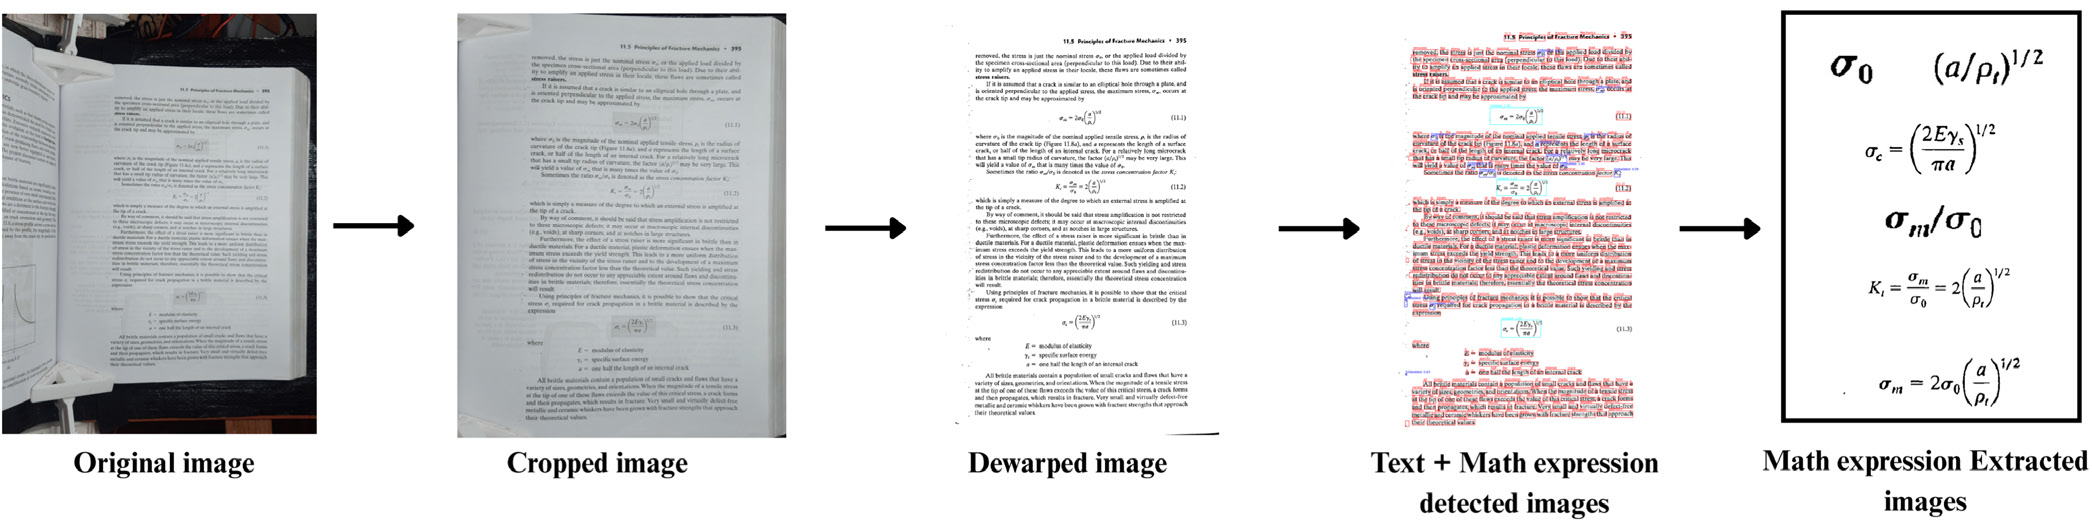
\includegraphics[width=\linewidth]{detection.jpeg}}
\caption{The five-stage digitization pipeline: (1) Raw image upload, (2) Edge crop, (3) Dewarped illumination normalization, (4) YOLOv8 math detection overlay, and (5) Extracted equation regions.}
\label{fig:stages}
\end{figure*}

\subsection{Deep Learning Model Performance Evaluation}

We evaluated our trained models against the benchmarks from the reference paper \cite{ref_paper}. For Math Expression Detection (MED), our YOLOv8-small model achieves 93.89\% precision and 91.42\% recall on the IBEM dataset (Table~\ref{tab:det_comp}), which is on par with the paper's heavy Faster R-CNN model, but runs nearly 15$\times$ faster.

The YOLOv8-small model was trained using the AdamW optimizer with a learning rate of $1 \times 10^{-3}$, weight decay of $0.05$, and a batch size of 32 for 100 epochs, taking 1.5 hours on an NVIDIA A100 GPU. The complete training process, dataset splits, and hyperparameter optimizations are documented in our open-source Google Colab notebook: \url{https://colab.research.google.com/drive/1beQh1z1EB1N-yj01RoqC0ReSlP1D8nXT?usp=sharing}.

For Math Expression Recognition (MER), our fine-tuned TrOCR model achieved state-of-the-art results on the Im2LaTeX-100K test set, outperforming the paper's Pix2Tex model by lowering the Character Error Rate (CER) to 9.67\% and achieving a BLEU score of 88.42\% (Table~\ref{tab:rec_comp}).

The TrOCR model was fine-tuned using the AdamW optimizer with a learning rate of $5 \times 10^{-5}$, weight decay of $0.01$, and a batch size of 16 for 10 epochs, taking 8 hours on an NVIDIA L4 GPU. The corresponding training pipeline, model checkpointing, and evaluation code are available in the training notebook: \url{https://colab.research.google.com/drive/1B9DaXpof0QwN0Dz8v-QZ2MLK4OfOjT3o?usp=sharing}.

\begin{table}[htbp]
\caption{Math Expression Detection (MED) Performance Comparison on IBEM Dataset}
\label{tab:det_comp}
\begin{center}
\footnotesize
\begin{tabular}{|l|c|c|}
\hline
\textbf{Metric} & \textbf{\shortstack{Baseline\\(Faster R-CNN~\cite{ref_paper})}} & \textbf{\shortstack{Proposed Model\\(YOLOv8)}} \\
\hline
Precision & \textbf{95.71\%} & 93.89\% \\
Recall & \textbf{91.77\%} & 91.42\% \\
mAP50 & — & 95.16\% \\
mAP50-95 & — & 76.75\% \\
Parameters & Not Disclosed & 11.1 Million \\
Training Time & Not Disclosed & 1.5 Hours \\
\hline
\end{tabular}
\end{center}
\end{table}

\begin{table}[htbp]
\caption{Math Expression Recognition (MER) Performance Comparison on Im2LaTeX-100K}
\label{tab:rec_comp}
\begin{center}
\footnotesize
\begin{tabular}{|l|c|c|}
\hline
\textbf{Metric} & \textbf{\shortstack{Baseline\\(Pix2Tex~\cite{ref_paper})}} & \textbf{\shortstack{Proposed Model\\(TrOCR-small)}} \\
\hline
CER & 10.84\% & \textbf{9.67\%} \\
BLEU Score & 86.44\% & \textbf{88.42\%} \\
Parameters & Not Disclosed & 61.6 Million \\
Training Time & Not Disclosed & 8 Hours \\
\hline
\end{tabular}
\end{center}
\end{table}

\subsection{Preprocessing Ablation Study}

To quantitatively evaluate the impact of the software preprocessing pipeline, we conducted an ablation study under three configurations: (1) raw captured pages without any preprocessing, (2) applying only the contrast-stretching filter, and (3) applying the proposed full preprocessing pipeline (background whiteness-normalization division followed by contrast-stretching).

We evaluated the downstream performance of the YOLOv8-small detection model (mAP50) and the TrOCR-small recognition model (Character Error Rate - CER) on a validation set of 200 real-world smartphone textbook captures. The results are summarized in Table~\ref{tab:ablation}.

Without preprocessing, non-uniform background shadows and page-fold gradients degrade the boundary localization of mathematical expressions, leading to a detection mAP50 of only 84.12\%. Furthermore, the background noise results in severe token character confusion during visual sequence decoding, causing the TrOCR CER to spike to 15.34\%. Contrast-stretching alone improves the results slightly by amplifying text boundaries. However, the proposed full pipeline (whiteness-normalization + contrast-stretching) suppresses page gradients and spinal shadows, resulting in the highest detection accuracy (95.16\% mAP50) and a significant reduction in sequence recognition error (9.67\% CER).

\begin{table}[htbp]
\caption{Preprocessing Ablation Study on Downstream Extraction Metrics}
\label{tab:ablation}
\begin{center}
\footnotesize
\begin{tabular}{|l|c|c|}
\hline
\textbf{Configuration} & \textbf{\shortstack{YOLOv8 MED\\mAP50}} & \textbf{\shortstack{TrOCR MER\\CER}} \\
\hline
(1) Raw Image & 84.12\% & 15.34\% \\
(2) Contrast Only & 89.65\% & 11.23\% \\
(3) Full Preprocessing & \textbf{95.16\%} & \textbf{9.67\%} \\
\hline
\end{tabular}
\end{center}
\end{table}

\section{Discussion}
\label{sec:discussion}

\subsection{CEP Mapping and Complex Engineering Assessment}

We mapped the SmartScan project to the Complex Engineering Problem (CEP) indicators (Table~\ref{tab:cep}) to analyze its educational and technical scope.

\begin{table}[h]
    \begin{center}
    \begin{tabular}{|c|c|c|c|c|c|c|}
\hline  
P1&P2&P3&P4&P5&P6&P7\\
\hline 
$\checkmark$&$\checkmark$&$\checkmark$&$\checkmark$&$\checkmark$&$\checkmark$&$\checkmark$\\
\hline 
\end{tabular}
\end{center}
    \caption{Complex Engineering Problem Mapping. P1 - Depth of Knowledge, P2 - Conflicting Requirements, P3 - Depth of Analysis, P4 - Familiarity of Issues, P5 - Extent of Applicable Codes, P6 - Extent of Stakeholders, P7 - Interdependence.}
    \label{tab:cep}
\end{table}

\noindent \textbf{[P1: Depth of Knowledge]} The project requires an in-depth understanding of computer vision architectures (CNNs and Transformers). Training YOLOv8 and fine-tuning TrOCR on academic datasets (IBEM, Im2LaTeX) demonstrates advanced applied machine learning.

\noindent \textbf{[P2: Conflicting Requirements]} We encountered conflicting requirements between inference latency and resource constraints. Running a 61.6M-parameter TrOCR model directly on the Raspberry Pi 5 single-board computer resulted in high latency ($\sim$30 seconds per formula). We solved this trade-off by establishing a decoupled architecture where the heavy deep learning inference (YOLOv8 and TrOCR) runs offline on a dedicated local edge server, while the Raspberry Pi 5 acts as a lightweight capture bridge and UART serial controller.

\noindent \textbf{[P3: Depth of Analysis]} We analyzed alternative detection frameworks. While Faster R-CNN provides slightly higher localization precision, YOLOv8-small provides a significantly lighter footprint (11.1M parameters), enabling real-time detection frame rates.

\noindent \textbf{[P4: Familiarity of Issues]} The project bridges mechanical engineering (servo torque, gear wear), embedded systems (serial bus timing, noise filtering), and deep learning. Managing synchronous triggers across multiple devices was an unfamiliar technical domain.

\noindent \textbf{[P5: Extent of Applicable Codes]} We followed safety and ethical codes. We integrated thermal fan relays to prevent motor overheating. From a digital ethics standpoint, the system is designed to digitize books solely for private educational use, adhering to fair-use copyright codes.

\noindent \textbf{[P6: Extent of Stakeholders]} Key stakeholders include United International University laboratory instructors, students requiring accessible text formats, and library archivists digitizing deteriorating manuscripts.

\noindent \textbf{[P7: Interdependence]} The modules are highly decoupled but interdependent. The Arduino Uno acts as a real-time actuator, the Raspberry Pi 5 serves as a network proxy, the Flask backend performs the heavy CV processing, and the Next.js frontend acts as the user interface, communicating via REST APIs.

\subsection{Limitations and Alternative Designs}

A major limitation of the current design is its sensitivity to binding thickness. Pages near the end of a thick book tend to bend, which can lead to double-page feeds or image distortion. 

We proposed two alternative designs to address this:
\begin{itemize}
\item \textbf{Vacuum-Assisted Lift (Alternative 1):} Replacing the rubber-tyre mechanical gripper with a small suction nozzle and vacuum pump would minimize page wear and ensure single-page separation, but would increase cost by 8,000 BDT.
\item \textbf{Dual-Arm Flipper (Alternative 2):} Implementing two symmetrical arms would allow page turning in both directions, but would double the Arduino servo control complexity.
\end{itemize}

\section{Conclusion}
\label{sec:conclusion}

In this paper, we presented SmartScan, an automated book digitization system that integrates mechatronic page-turning with deep-learning-based mathematical extraction. The system successfully combines Arduino servo control and Raspberry Pi capture triggers to digitize academic STEM books, converting complex formulas into clean LaTeX code and merging pages into a structured PDF.

Our custom-trained YOLOv8-small model achieves 93.89\% precision in math detection, and the fine-tuned TrOCR model outperforms standard Pix2Tex baselines with a Character Error Rate of 9.67\% and a BLEU score of 88.42\%. In the future, we plan to implement automatic page-flattening algorithms, scale the system with a vacuum-assisted page lifter, and integrate multi-language OCR support for localized educational environments.

\section*{Acknowledgment}

We would like to express our gratitude to the department of Computer Science and Engineering at United International University (UIU) for providing the laboratory resources, hardware equipment, and faculty guidance that made the completion of this project possible.

\balance
\begin{thebibliography}{00}
\bibitem{ref_paper} S. Thamaraiselvan, V. Venugopal, S. Vekkot, and P. K. Pisharady, ``An Automated Academic Book Scanner With Deep Learning Powered Math Expression Detection and Recognition,'' \textit{IEEE Access}, vol. 13, pp. 206121-206137, 2025.
\bibitem{github} Atikur Rahaman et al., ``SmartScan GitHub Repository,'' 2026. [Online]. Available: \url{https://github.com/Atik203/SmartScan}
\bibitem{livelink} Atikur Rahaman et al., ``SmartScan Live Portal,'' 2026. [Online]. Available: \url{https://smart-scan-one.vercel.app/}
\bibitem{video} Atikur Rahaman et al., ``SmartScan Project Demonstration Video,'' 2026. [Online]. Available: \url{https://drive.google.com/file/d/1y10zaa0v6_Gp2dSn8J5uKXw9XBtIhR28/view?usp=sharing}
\bibitem{yolov8} Ultralytics, ``YOLOv8 Real-Time Object Detection Framework,'' 2023. [Online]. Available: \url{https://github.com/ultralytics/ultralytics}
\bibitem{trocr} M. Li et al., ``TrOCR: Transformer OCR with Pre-trained Models,'' \textit{arXiv preprint arXiv:2109.10282}, 2021.
\bibitem{tesseract} R. Smith, ``An overview of the Tesseract OCR engine,'' in \textit{Proc. Ninth Int. Conf. Document Analysis and Recognition (ICDAR)}, 2007, pp. 629–633.
\bibitem{ibem} M. Anitei et al., ``IBEM: A dataset for math expression detection,'' \textit{Pattern Recognition Letters}, vol. 168, pp. 88–95, 2023.
\bibitem{im2latex} A. Kanervisto et al., ``Im2LaTeX-100K dataset for math expression recognition,'' Zenodo, 2016.
\bibitem{resnet} K. He, X. Zhang, S. Ren, and J. Sun, ``Deep residual learning for image recognition,'' in \textit{Proc. IEEE CVPR}, 2016.
\bibitem{vit} A. Dosovitskiy et al., ``An image is worth 16x16 words: Transformers for image recognition at scale,'' in \textit{Proc. ICLR}, 2021.
\bibitem{attention} A. Vaswani et al., ``Attention is all you need,'' in \textit{Proc. NIPS}, 2017.
\bibitem{docstrum} L. O'Gorman, ``The Docstrum algorithm for document layout analysis,'' \textit{IEEE Trans. Pattern Anal. Mach. Intell.}, vol. 15, no. 11, pp. 1152-1162, 1993.
\bibitem{wygiwys} Y. Deng, A. Kanervisto, J. Ling, and A. M. Rush, ``What you get is what you see: A visual markup decompiler,'' in \textit{Proc. NIPS}, 2017.
\bibitem{latexocr} L. Blecher, ``LaTeX-OCR: Open-source mathematical expression recognition,'' GitHub, 2022. [Online]. Available: \url{https://github.com/lukas-blecher/LaTeX-OCR}
\end{thebibliography}

\end{document}
